\documentclass[tikz,border=8pt]{standalone}
% Shared look for every TikZ diagram. Load with % Shared look for every TikZ diagram. Load with % Shared look for every TikZ diagram. Load with \input{../../tools/tikz-style.tex}
\usepackage[T1]{fontenc}
\usepackage{lmodern}
\renewcommand{\sfdefault}{lmr}  % diagrams use the same serif as the text
\usetikzlibrary{arrows.meta, positioning, shapes.geometric, calc, fit, backgrounds}
\definecolor{cblue}{HTML}{4C78A8}
\definecolor{corange}{HTML}{F58518}
\definecolor{cgreen}{HTML}{54A24B}
\definecolor{cred}{HTML}{E45756}
\definecolor{cpurple}{HTML}{B279A2}
\definecolor{cgrey}{HTML}{6B6B6B}
\tikzset{
  every picture/.style={font=\sffamily, line width=1.2pt},
  box/.style={draw=#1, fill=#1!12, rounded corners=4pt, align=center, inner sep=7pt, minimum height=1.1cm},
  box/.default=cgrey,
  arrow/.style={-{Stealth[length=3mm]}, draw=cgrey, line width=1.4pt},
  title/.style={font=\sffamily\bfseries\Large},
  note/.style={font=\sffamily\small, text=cgrey, align=center},
}
\AtBeginDocument{\hyphenpenalty=10000 \exhyphenpenalty=10000}

\usepackage[T1]{fontenc}
\usepackage{lmodern}
\renewcommand{\sfdefault}{lmr}  % diagrams use the same serif as the text
\usetikzlibrary{arrows.meta, positioning, shapes.geometric, calc, fit, backgrounds}
\definecolor{cblue}{HTML}{4C78A8}
\definecolor{corange}{HTML}{F58518}
\definecolor{cgreen}{HTML}{54A24B}
\definecolor{cred}{HTML}{E45756}
\definecolor{cpurple}{HTML}{B279A2}
\definecolor{cgrey}{HTML}{6B6B6B}
\tikzset{
  every picture/.style={font=\sffamily, line width=1.2pt},
  box/.style={draw=#1, fill=#1!12, rounded corners=4pt, align=center, inner sep=7pt, minimum height=1.1cm},
  box/.default=cgrey,
  arrow/.style={-{Stealth[length=3mm]}, draw=cgrey, line width=1.4pt},
  title/.style={font=\sffamily\bfseries\Large},
  note/.style={font=\sffamily\small, text=cgrey, align=center},
}
\AtBeginDocument{\hyphenpenalty=10000 \exhyphenpenalty=10000}

\usepackage[T1]{fontenc}
\usepackage{lmodern}
\renewcommand{\sfdefault}{lmr}  % diagrams use the same serif as the text
\usetikzlibrary{arrows.meta, positioning, shapes.geometric, calc, fit, backgrounds}
\definecolor{cblue}{HTML}{4C78A8}
\definecolor{corange}{HTML}{F58518}
\definecolor{cgreen}{HTML}{54A24B}
\definecolor{cred}{HTML}{E45756}
\definecolor{cpurple}{HTML}{B279A2}
\definecolor{cgrey}{HTML}{6B6B6B}
\tikzset{
  every picture/.style={font=\sffamily, line width=1.2pt},
  box/.style={draw=#1, fill=#1!12, rounded corners=4pt, align=center, inner sep=7pt, minimum height=1.1cm},
  box/.default=cgrey,
  arrow/.style={-{Stealth[length=3mm]}, draw=cgrey, line width=1.4pt},
  title/.style={font=\sffamily\bfseries\Large},
  note/.style={font=\sffamily\small, text=cgrey, align=center},
}
\AtBeginDocument{\hyphenpenalty=10000 \exhyphenpenalty=10000}

% Section 3: the 2-2-1 network with all 9 trainable parameters named. 4 + 2 in layer 1, 2 + 1 in layer 2.
\begin{document}
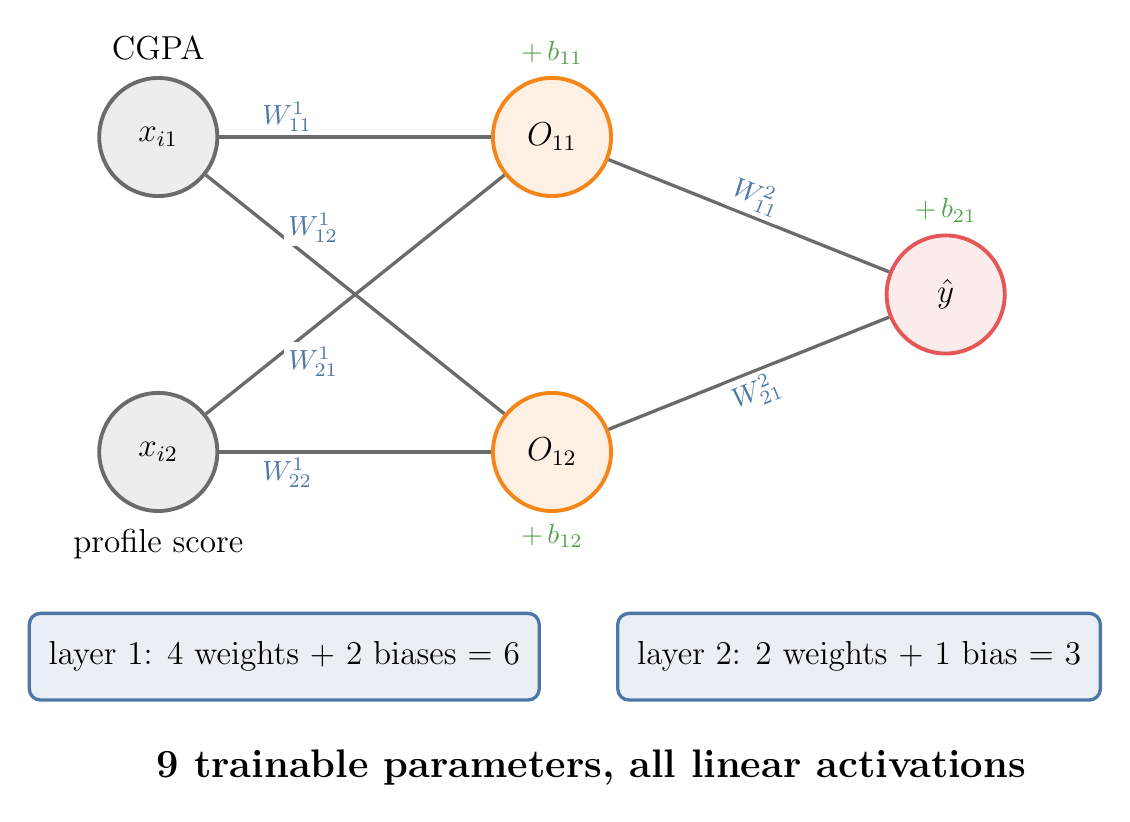
\begin{tikzpicture}[n/.style={circle, draw=#1, fill=#1!12, minimum size=1.5cm, font=\large, line width=1.4pt},
                    w/.style={font=\normalsize, fill=white, inner sep=1.5pt, text=cblue},
                    e/.style={draw=cgrey, line width=1.2pt}]
  \node[n=cgrey] (x1) at (0, 2) {$x_{i1}$};
  \node[n=cgrey] (x2) at (0, -2) {$x_{i2}$};
  \node[n=corange] (h1) at (5, 2) {$O_{11}$};
  \node[n=corange] (h2) at (5, -2) {$O_{12}$};
  \node[n=cred] (o) at (10, 0) {$\hat y$};
  \node[note, font=\large, text=black, above=2pt of x1] {CGPA};
  \node[note, font=\large, text=black, below=2pt of x2] {profile score};
  \draw[e] (x1) -- node[w, pos=0.25, above] {$W^{1}_{11}$} (h1);
  \draw[e] (x2) -- node[w, pos=0.25, below] {$W^{1}_{22}$} (h2);
  \draw[e] (x1) -- node[w, pos=0.22, right=4pt] {$W^{1}_{12}$} (h2);
  \draw[e] (x2) -- node[w, pos=0.22, right=4pt] {$W^{1}_{21}$} (h1);
  \draw[e] (h1) -- node[w, above, sloped] {$W^{2}_{11}$} (o);
  \draw[e] (h2) -- node[w, below, sloped] {$W^{2}_{21}$} (o);
  \node[w, text=cgreen, above=2pt of h1] {$+\,b_{11}$};
  \node[w, text=cgreen, below=2pt of h2] {$+\,b_{12}$};
  \node[w, text=cgreen, above=2pt of o] {$+\,b_{21}$};
  \node[box=cblue, font=\large, align=center] at (1.6, -4.6) {layer 1: 4 weights + 2 biases = 6};
  \node[box=cblue, font=\large, align=center] at (8.9, -4.6) {layer 2: 2 weights + 1 bias = 3};
  \node[title] at (5.5, -6.0) {9 trainable parameters, all linear activations};
\end{tikzpicture}
\end{document}
